%%%%%%%%%%%%%%%%%%%%%%%%%%%%%%%%%%%%%%%%%
% Beamer Presentation
% LaTeX Template
% Version 1.0 (10/11/12)
%
% This template has been downloaded from:
% http://www.LaTeXTemplates.com
%
% License:
% CC BY-NC-SA 3.0 (http://creativecommons.org/licenses/by-nc-sa/3.0/)
%
%%%%%%%%%%%%%%%%%%%%%%%%%%%%%%%%%%%%%%%%%

%----------------------------------------------------------------------------------------
%	PACKAGES AND THEMES
%----------------------------------------------------------------------------------------

\documentclass{beamer}

\mode<presentation> {

% The Beamer class comes with a number of default slide themes
% which change the colors and layouts of slides. Below this is a list
% of all the themes, uncomment each in turn to see what they look like.

\usetheme{default}
%\usetheme{AnnArbor}
%\usetheme{Antibes}
%\usetheme{Bergen}
%\usetheme{Berkeley}
%\usetheme{Berlin}
%\usetheme{Boadilla}
%\usetheme{CambridgeUS}
%\usetheme{Copenhagen}
%\usetheme{Darmstadt}
%\usetheme{Dresden}
%\usetheme{Frankfurt}
%\usetheme{Goettingen}
%\usetheme{Hannover}
%\usetheme{Ilmenau}
%\usetheme{JuanLesPins}
%\usetheme{Luebeck}
%\usetheme{Madrid}
%\usetheme{Malmoe}
%\usetheme{Marburg}
%\usetheme{Montpellier}
%\usetheme{PaloAlto}
%\usetheme{Pittsburgh}
%\usetheme{Rochester}
%\usetheme{Singapore}
%\usetheme{Szeged}
%\usetheme{Warsaw}

% As well as themes, the Beamer class has a number of color themes
% for any slide theme. Uncomment each of these in turn to see how it
% changes the colors of your current slide theme.

%\usecolortheme{albatross}
%\usecolortheme{beaver}
%\usecolortheme{beetle}
%\usecolortheme{crane}
%\usecolortheme{dolphin}
%\usecolortheme{dove}
%\usecolortheme{fly}
%\usecolortheme{lily}
%\usecolortheme{orchid}
%\usecolortheme{rose}
%\usecolortheme{seagull}
%\usecolortheme{seahorse}
%\usecolortheme{whale}
%\usecolortheme{wolverine}

%\setbeamertemplate{footline} % To remove the footer line in all slides uncomment this line
%\setbeamertemplate{footline}[page number] % To replace the footer line in all slides with a simple slide count uncomment this line

%\setbeamertemplate{navigation symbols}{} % To remove the navigation symbols from the bottom of all slides uncomment this line
}

\usepackage{graphicx} % Allows including images
\usepackage{booktabs} % Allows the use of \toprule, \midrule and \bottomrule in tables

%----------------------------------------------------------------------------------------
%	TITLE PAGE
%----------------------------------------------------------------------------------------

\title[Short title]{Generalized estimating equation modeling on correlated microbiome sequencing data with longitudinal measures} % The short title appears at the bottom of every slide, the full title is only on the title page

\author{Emily Palmer} % Your name
\institute[OSU] % Your institution as it will appear on the bottom of every slide, may be shorthand to save space
{
Journal Club, Oregon State University  %\\ % Your institution for the title page
%\medskip
%\textit{john@smith.com} % Your email address
}
\date{\today} % Date, can be changed to a custom date

\begin{document}

\begin{frame}
\titlepage % Print the title page as the first slide
\end{frame}

\begin{frame}
\frametitle{Overview} % Table of contents slide, comment this block out to remove it
\tableofcontents % Throughout your presentation, if you choose to use \section{} and \subsection{} commands, these will automatically be printed on this slide as an overview of your presentation
\end{frame}

%----------------------------------------------------------------------------------------
%	PRESENTATION SLIDES
%----------------------------------------------------------------------------------------

%------------------------------------------------
\section{Introduction} % Sections can be created in order to organize your presentation into discrete blocks, all sections and subsections are automatically printed in the table of contents as an overview of the talk
%------------------------------------------------

%\subsection{Subsection Example} % A subsection can be created just before a set of slides with a common theme to further break down your presentation into chunks

\begin{frame}
\frametitle{Introduction}
\begin{itemize}
  \item Estimate correlations between multiple OTUs
  \item Encorporate correlations into models with longitudinal OTU measures
  \item Estimate predictors effects and OTU measures
  \item Two-part Microbiome Taxonomic Longitudinal Correlation (MLTC) model
\end{itemize}
\end{frame}


\section{Correlation strucutre}
\subsection{Taxonomic structure of OTUs}

\begin{frame}[t]{Notation and Definitions}
  \begin{itemize}
    \item $N$ OTUs
    \item $I$ levels:
    \begin{itemize}
      \item 1st taxonomic level is the level at which all observed $N$ OTUs belong to the same taxon but not at one level lower
    \end{itemize}
    \item $M_i$: number of taxa at level $i$ ($M_1 = 1, M_I = N$)
    \item $t_{m_i, i}$: taxon at level $i$
    \item $n_{m_i, i}$: number of OTUs belonging to taxon $t_{m_i,i}$
  \end{itemize}
\end{frame}
%--- Next Frame ---%


%--- Next Frame ---%


\begin{frame}
\frametitle{Example}

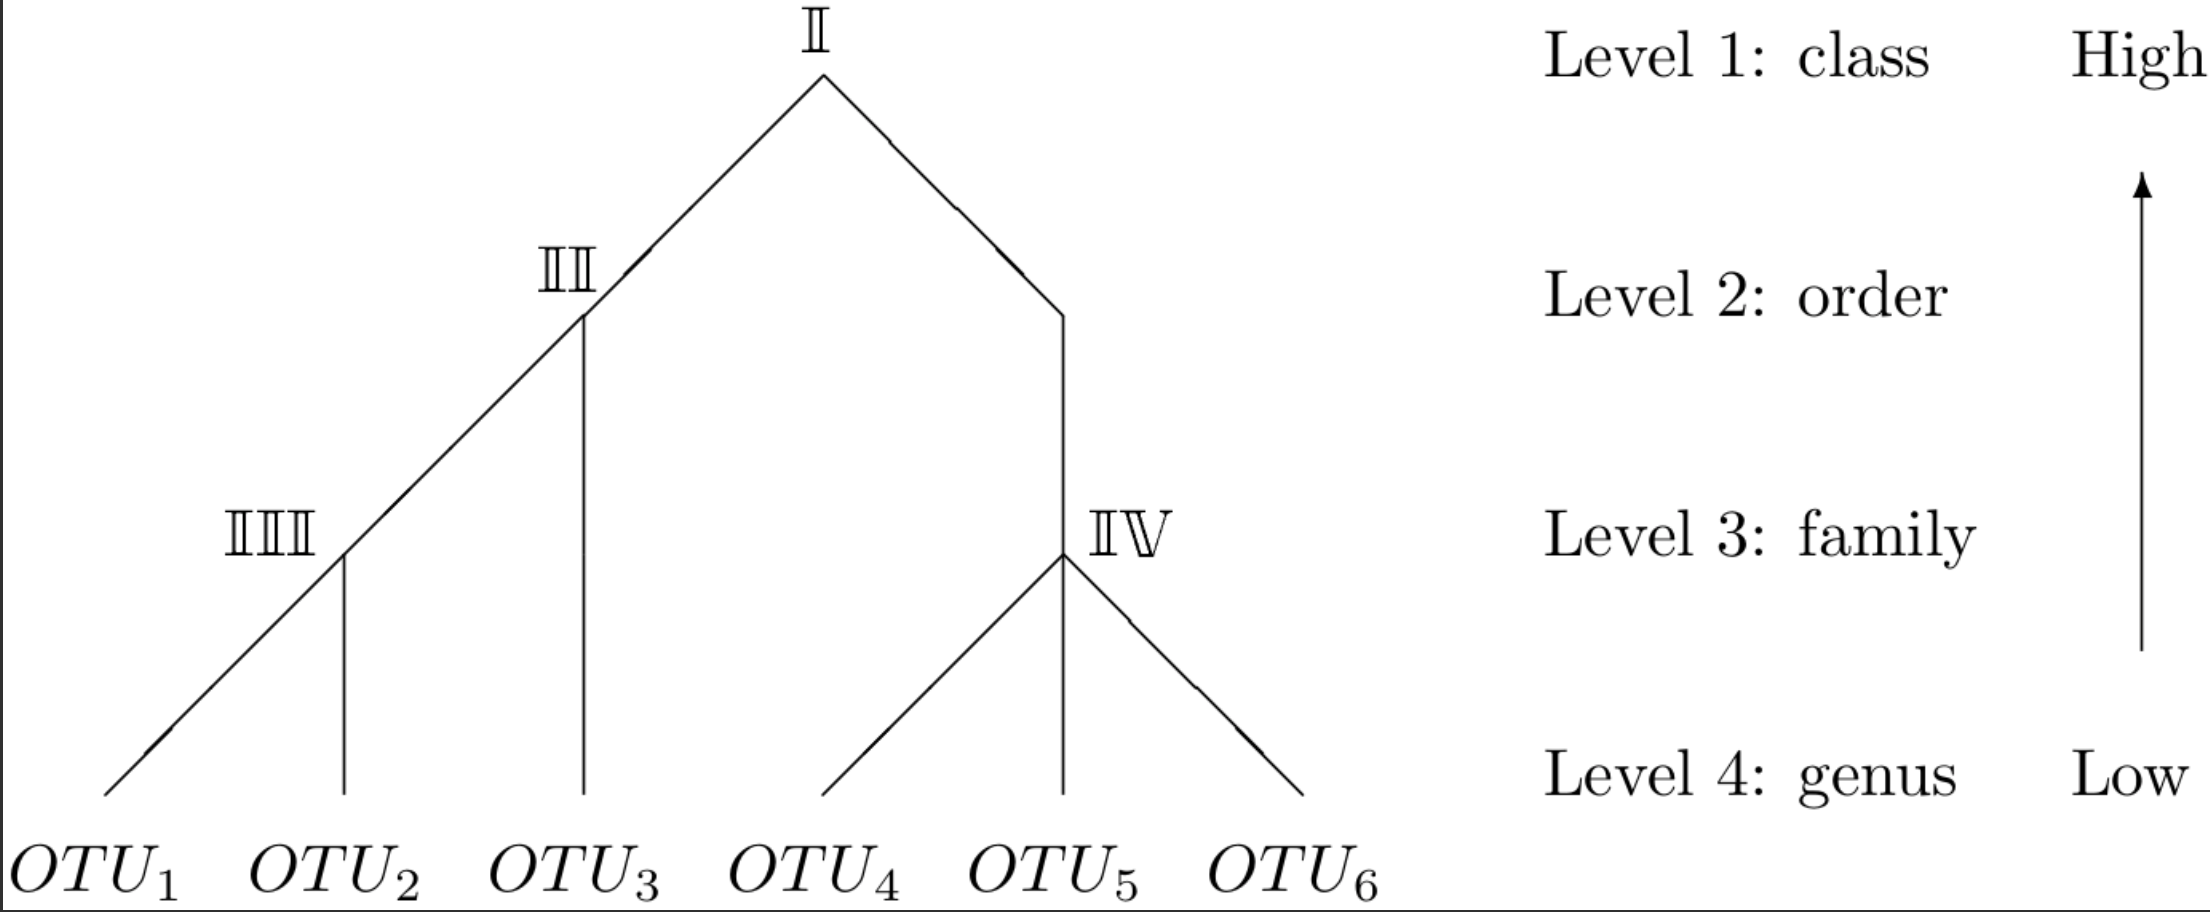
\includegraphics[width = \textwidth]{otu_tree.png}

\end{frame}

%------------------------------------------------

\begin{frame}[t]{Correlation matrix of taxonomic structure - Assumptions}
  \begin{itemize}
    \item Assume that OTUs that belong to the same taxa at some higher level have some correlation
    \item From taxonomic structure, all OTUs will belong to same taxa at hightest level, so there are $\binom{N}{2}$ possible correlations - infeasible to model
    \item Clusters of OTUs (otus belonging to the same taxa)
    \item Assume that two pairs of OTUs have the same correlation if the first common taxa of both pairs are identical

    If $\mathcal{P}^*$ and $\mathcal{P}^\dagger$ are two pairs of OTUs, with correlation $\rho^*$ and $\rho^\dagger$. $t_{m_i^*, i^*}$ is first common taxa of $\mathcal{P}^*$ $t_{m_i^\dagger, i^\dagger}$ is first common taxa of $\mathcal{P}^\dagger$

    $$\rho^* = \rho^\dagger \leftrightarrow t_{m_i^*, i^*} = t_{m_i^\dagger, i^\dagger}$$
  \end{itemize}
\end{frame}
%--- Next Frame ---%




\begin{frame}[t]{Finding the taxonomic structure matrix}
  \begin{itemize}
    \item The taxonomic structure matrix
    \item Go through algoritm...
  \end{itemize}
\end{frame}
%--- Next Frame ---%



\subsection{Modelling correlations from repeated measures}

\begin{frame}[t]{Correlations of longitudinal data }
  Types of correlations between pairs of time points
  \begin{itemize}
    \item Exchangable
    \begin{itemize}
      \item Assumes all correlations are equal to each other
    \end{itemize}
    \item Toeplitz
    \begin{itemize}
      \item Assumes time points with equal temporal distance have equal correlation
    \end{itemize}
    \item Unstructured
    \begin{itemize}
      \item Assumes each pair has a different correlations
      \item Most complicated structure for correlation parameter estimation
    \end{itemize}
  \end{itemize}
  Correlation structure matrix for the the same individual is dentoed $\Omega_T$
\end{frame}
%--- Next Frame ---%


\begin{frame}
\frametitle{Example}

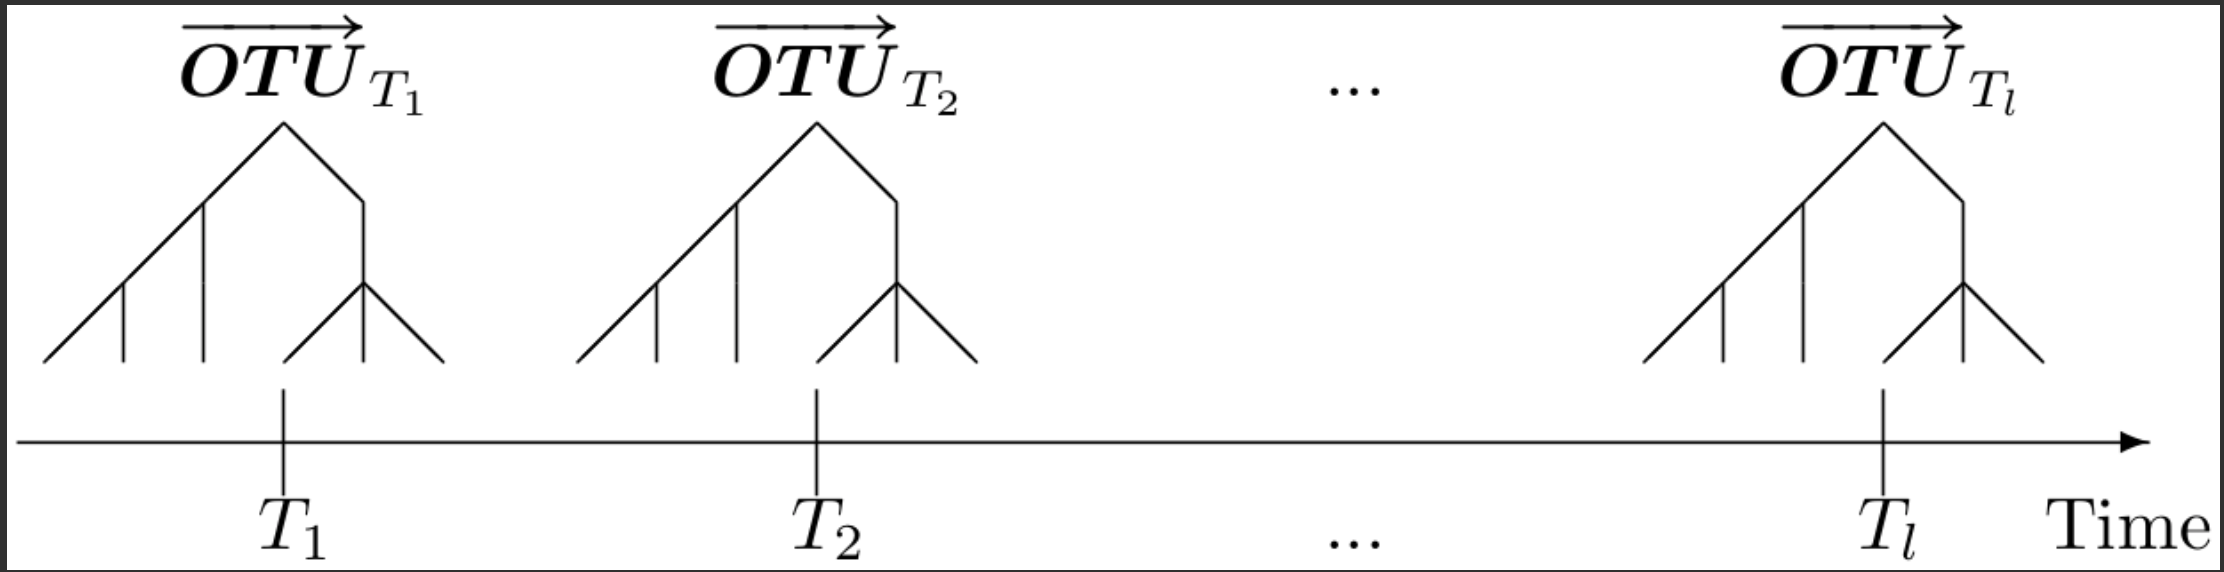
\includegraphics[width = \textwidth]{otu_time_tree.png}

\end{frame}

\begin{frame}
\frametitle{Multiple Columns}
Example for 3 timepoints
\begin{columns}[c] % The "c" option specifies centered vertical alignment while the "t" option is used for top vertical alignment

\column{.45\textwidth} % Left column and width
\textbf{Exchangable structure}
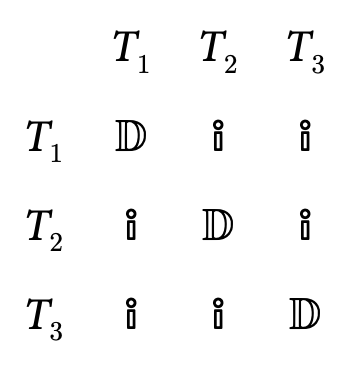
\includegraphics[width = \textwidth]{exchangeable.png}


\column{.5\textwidth} % Right column and width
\textbf{Toeplitz structure}
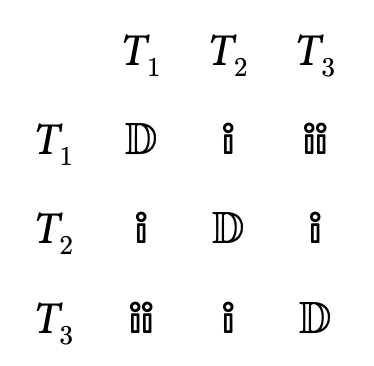
\includegraphics[width = \textwidth]{toeplitz.png}

\end{columns}
\end{frame}


\begin{frame}[t]{Combining longitudinal and sample correlation}

When both longitudinal and sample correlations exist, the repeated measure correlation matrix is all combinations of time points and repeated samples

  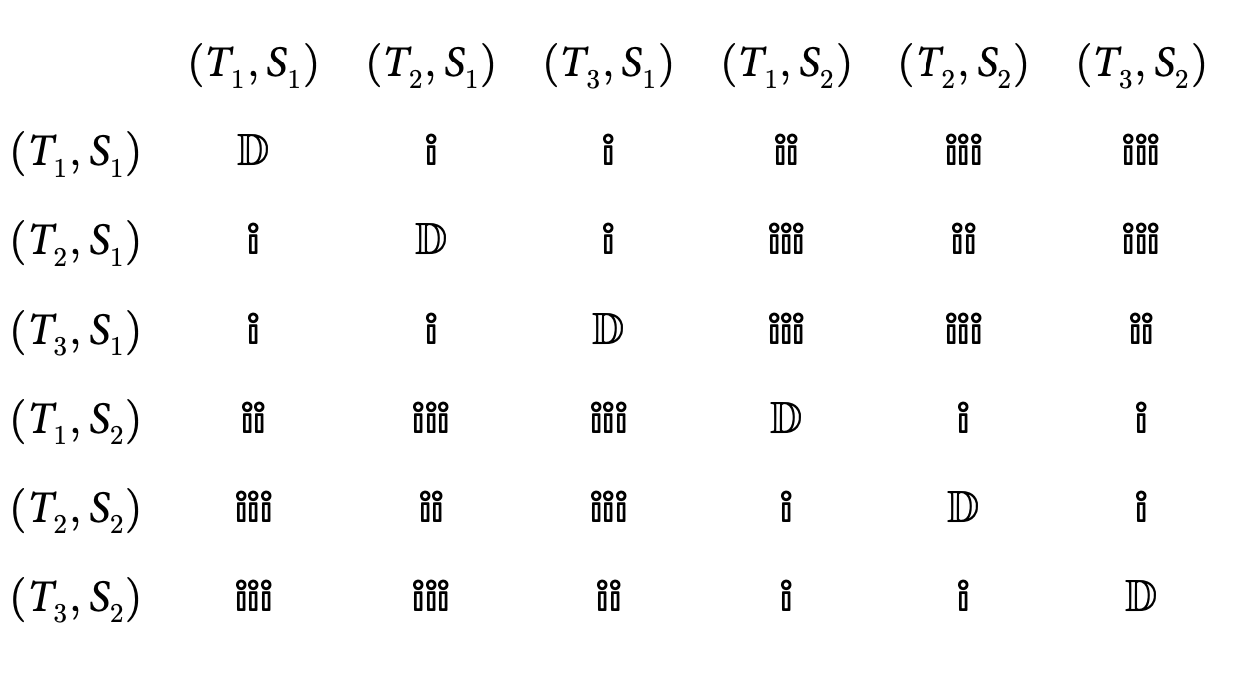
\includegraphics[width = \textwidth]{longitudinal_sample.png}

\end{frame}


\subsection{Integrative Correlation Matrix}
\begin{frame}[t]{Integrative Correlation Matrix }
  \begin{columns}[c] % The "c" option specifies centered vertical alignment while the "t" option is used for top vertical alignment

  \column{.45\textwidth} % Left column and width
  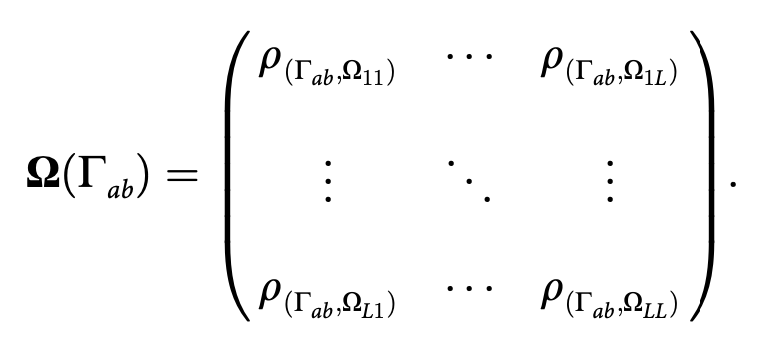
\includegraphics[width = \textwidth]{omega_gamma.png}
  \column{.5\textwidth} % Right column and width
  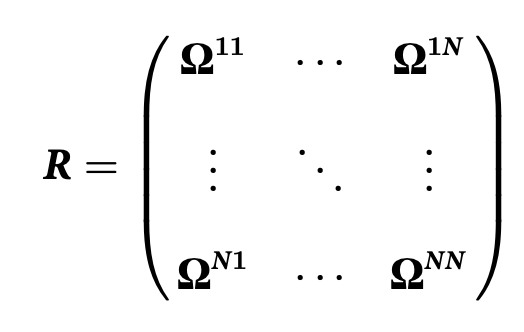
\includegraphics[width = \textwidth]{R.png}

Dimention of $R = (N \times L) \times (N \times L)$

Diagonals of $R = \rho(\mathbb{D},\mathbb{D})$ are 1, off-diagonals need to be estimated

  \end{columns}
\end{frame}


\section{Microbiome Taxonomic Longitudinal Correlation model}


\begin{frame}[t]{Introduction to MTLC:}
  MTLC:
  \begin{itemize}
    \item Estimate predictor effects
    \item Estimate correlation coefficients between OTUs, longitudinal measures and other repeated measures
    \item Perform hypothesis testing of predictor effects
  \end{itemize}
\end{frame}

\subsection{GEE framework}

\begin{frame}[t]{Generalized estimating equation framework}
  \begin{itemize}
    \item $y_k$ independent clusters $k = 1, \ldots , K$
    \item $J_k$ cluster length for cluster $y_k = (y_{k1}, \ldots , y_{kJ_k})$
    \item $\mathbf{x}_{kj}$ the vector of covariates with length $p$
    \item $\boldsymbol\mu_k = (\mu_{k1}, \ldots , \mu_{kJ_k})$
    \item Each observation $y_{kj}$
    $$g(\mu_{kj}) = \mathbf{x}_{kj}'\boldsymbol\beta$$
    \item Conditional variance of $y_{kj}$
    $$\text{Var}(y_{kj}|\boldsymbol{x}_{kj}) = v(\boldsymbol \mu_{kj}\phi)$$
    $v$ is the variance function depending on the distribution of $y_{kj}$, $\phi$ is dispersion parameter
  \end{itemize}
%--- Next Frame ---%
\end{frame}


\begin{frame}[t]{cont}
  \begin{itemize}
    \item Estimate $\boldsymbol\beta$ by solving the generalized estimating equation
    $$U(\boldsymbol\beta) = \sum_{k = 1}^K \boldsymbol{D}_k'\boldsymbol{V}_{k}^{-1}(\boldsymbol{y}_k - \boldsymbol{\mu}_k) = 0$$
    \item $\boldsymbol{D}_k = \frac{d\mu_k}{d\beta}$, $\boldsymbol{V}_k = \boldsymbol{A}_k^{1/2}\boldsymbol{R}_k(\boldsymbol\rho)\boldsymbol{A}_k^{1/2}$,
    \item  $\boldsymbol{A}_k = diag(\mu_{k1}\phi, \ldots , \mu_{kJ_k}\phi)$ $\boldsymbol\rho$ collection of all correlation coefficients in $\boldsymbol{R_k}$
    \item $\phi, \boldsymbol\rho$ also need to be estimated
    $$\hat\phi = \frac{1}{\sum_{k=1}^K J_k - p}\sum_{k=1}^K\sum_{j=1}^{J_k} e^2_{kj}$$
    where $e_{kj}$ is the pearson residual
    \item $\hat{\boldsymbol\rho}$ is estimated as a funtion of $\phi$ and $e_{kj}$, depending on the correlation structure $R $
  \end{itemize}
\end{frame}


%--- Next Frame ---%

\begin{frame}[t]{Hypothesis testing}
  In GEE theory,
  $\hat{\boldsymbol \beta}$ is asymptotically normally distributed with mean $\boldsymbol \beta$ and variance
\end{frame}

%--- Next Frame ---%











%------------------------------------------------

\begin{frame}[fragile] % Need to use the fragile option when verbatim is used in the slide
\frametitle{Citation}
An example of the \verb|\cite| command to cite within the presentation:\\~

This statement requires citation \cite{p1}.
\end{frame}

%------------------------------------------------

\begin{frame}
\frametitle{References}
\footnotesize{
\begin{thebibliography}{99} % Beamer does not support BibTeX so references must be inserted manually as below
\bibitem[Smith, 2012]{p1} John Smith (2012)
\newblock Title of the publication
\newblock \emph{Journal Name} 12(3), 45 -- 678.
\end{thebibliography}
}
\end{frame}

%------------------------------------------------


%----------------------------------------------------------------------------------------

\end{document}
